\documentclass{beamer}
\usepackage{minted}
\usepackage[skins,minted,breakable]{tcolorbox}
\usepackage[english]{babel}
\usepackage{subcaption}
\usetikzlibrary{matrix,backgrounds}
\usepackage{multirow}
\usepackage{hyperref}
\usepackage{multicol}
\usepackage{adjustbox}
\usepackage{soul}
\usepackage{graphicx}% http://ctan.org/pkg/graphicx
\usepackage{booktabs}% http://ctan.org/pkg/booktabs

\graphicspath{ {./img/} }
\selectlanguage{english}
\usepackage[utf8]{inputenc}
\usetheme{PaloAlto}
\setbeamerfont{section in sidebar}{size=\fontsize{2}{4}\selectfont}
\setbeamerfont{subsection in sidebar}{size=\fontsize{2}{3}\selectfont}
\setbeamerfont{subsubsection in sidebar}{size=\fontsize{2}{2}\selectfont}

\setbeamerfont{section in toc}{size=\footnotesize}
\setbeamerfont{subsection in toc}{size=\scriptsize}
\setbeamerfont{subsubsection in toc}{size=\tiny}

\hypersetup{
    urlcolor=cyan           % color of external links
}

\title{Cloud Computing}
\date{$14^{th}$ March 2019}
\subtitle{Working with Google Cloud}

\author{Carlos Sánchez Páez}

\makeatletter
  \setbeamertemplate{sidebar \beamer@sidebarside}%{sidebar theme}
  {
    \beamer@tempdim=\beamer@sidebarwidth%
    \advance\beamer@tempdim by -6pt%
    \insertverticalnavigation{\beamer@sidebarwidth}%
    \vfill
    \ifx\beamer@sidebarside\beamer@lefttext%
    \else%
      \usebeamercolor{normal text}%
      \llap{\usebeamertemplate***{navigation symbols}\hskip0.1cm}%
      \vskip2pt%
    \fi%
}%
\makeatother

\subject{Cloud Computing}
\AtBeginSection[]
  {
     \begin{frame}<beamer>
     \frametitle{Index}
     \tableofcontents[currentsection]
     \end{frame}
  }
\AtBeginSubsection[]
{
  \begin{frame}<beamer>{Index}
    \tableofcontents[currentsection,currentsubsection]
  \end{frame}
}
\AtBeginSubsubsection[]
{
  \begin{frame}<beamer>{Index}
    \tableofcontents[currentsection,currentsubsection]
  \end{frame}
}

% Let's get started
\begin{document}
\centering
\begin{frame}
 \titlepage
\end{frame}

\begin{frame}{Index}
 \tableofcontents
 % You might wish to add the option [pausesections]
\end{frame}

\section{What is Google Cloud Platform?}

\begin{frame}[fragile]{What is Google Cloud Platform?}
  \begin{itemize}[<+->]
    \item Set of Google's computing resources.
    \item They are internally used by Google for their products.
    \item Number 3 in the public cloud market (behind AWS and Azure).
    \item Offers IaaS, PaaS, SaaS over more than 50 products.
  \end{itemize}
\end{frame}


\begin{frame}[fragile]{Main advantages}
  \begin{itemize}[<+->]
    \item You can freely choose the resources for your Virtual Machine or use a template.
    \item Lots of interactive tutorials.
    \item Project Control Panel.
    \item Android App.
    \item Online terminal or CLI available.
  \end{itemize}
\end{frame}

\section{Who uses it?}

\begin{frame}[fragile]{Who uses it?}
\begin{figure}[H]
  \centering
  
\includegraphics[scale=0.35]{logos.png}
\end{figure}
More than 4 million paying customers (February 2018).
\end{frame}

\section{Google Cloud Platform products}

\begin{frame}[fragile]{Google Cloud Platform products}
\begin{figure}[H]
  \centering
  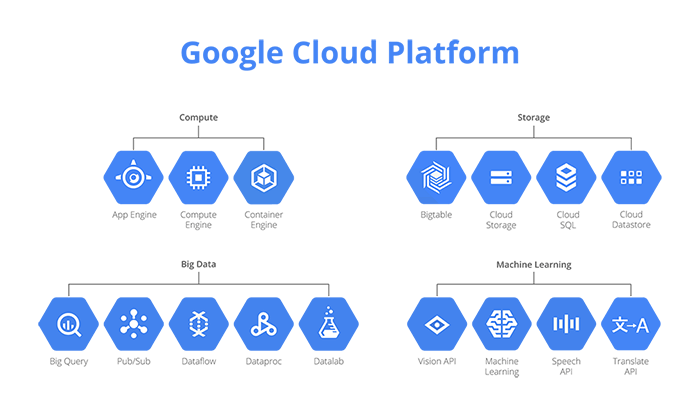
\includegraphics[width = \textwidth]{img/cloud_products}
\end{figure}

\end{frame}

\subsection{Computing}

\begin{frame}[fragile]{GCP Computing products}
  \begin{itemize}
    \item App Engine: scalable apps in a serverless platform (PaaS).
    \item Compute Engine: scalable virtual machines (IaaS).
    \item Kubernetes: run containers.
  \end{itemize}
\end{frame}

\subsection{Networking}

\begin{frame}[fragile]{GCP Networking products}
  \begin{itemize}
    \item Cloud Armor: protection against DoS attacks.
    \item Cloud VPN
    \item Network Service Tiers: optimize network for performance or cost.
    \item Load balancing: intelligent scaling through multiple regions.
  \end{itemize}
\end{frame}

\subsection{Big Data}

\begin{frame}[fragile]{GCP Big Data products}
  \begin{itemize}
    \item Dataflow: batch data processing.
    \item Genomics (for bioinformatics)
    \item Dataprep: clean data for analysis.
  \end{itemize}
\end{frame}

\subsection{Machine Learning}

\begin{frame}[fragile]{GCP Machine Learning products}
  \begin{itemize}
    \item Vision API: recognise objects in an image.
    \item Speech API: voice to text.
    \item Natural Language API: extract information from a text (sentiment, importance in the whole text).
    \item Translate API: Google Translate.
  \end{itemize}
\end{frame}

\section{Let's try it!}



\begin{frame}[fragile]{Source code}
  \begin{minted}{python}
  import webapp2
  class MainPage(webapp2.RequestHandler):
  def get(self):
      self.response.headers
      ['Content-Type'] = 'text/plain'
      self.response.write('Hello world!')

  app = webapp2.WSGIApplication([
  ('/', MainPage),
  ], debug=True)


  \end{minted}
\end{frame}

\begin{frame}[fragile]{Step 1: creating the project}
    \begin{figure}[H]
      \centering
      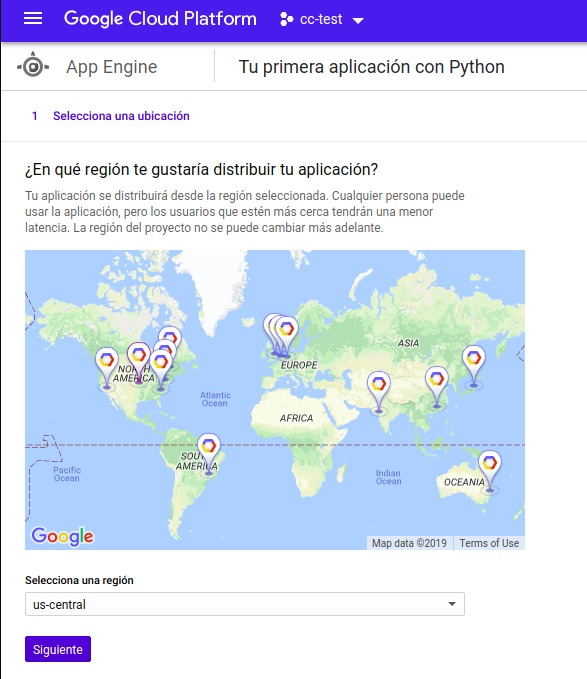
\includegraphics[scale=0.4]{img/tutorial/1select_region}
    \end{figure}
\end{frame}

\begin{frame}[fragile]{Control panel}
    \begin{figure}[H]
      \centering
      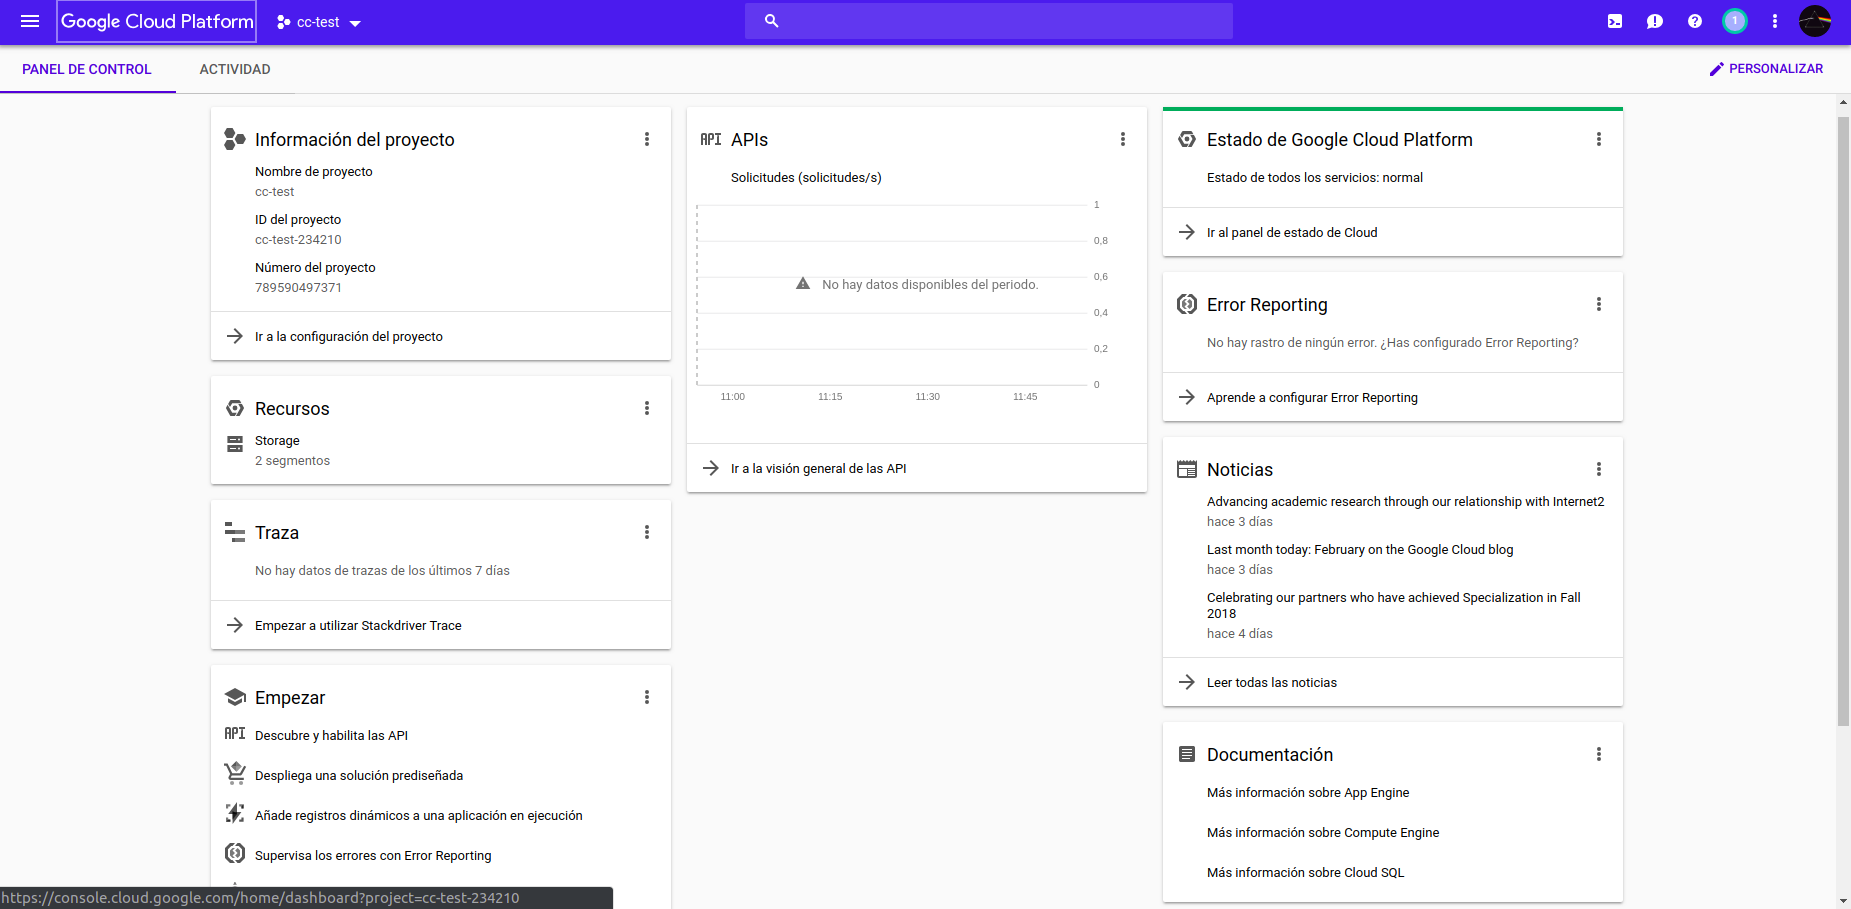
\includegraphics[scale=0.2]{img/tutorial/2controlpanel}
    \end{figure}
\end{frame}

\begin{frame}[fragile]{Step 2: setting the project in gcloud CLI}
    \begin{figure}[H]
      \centering
      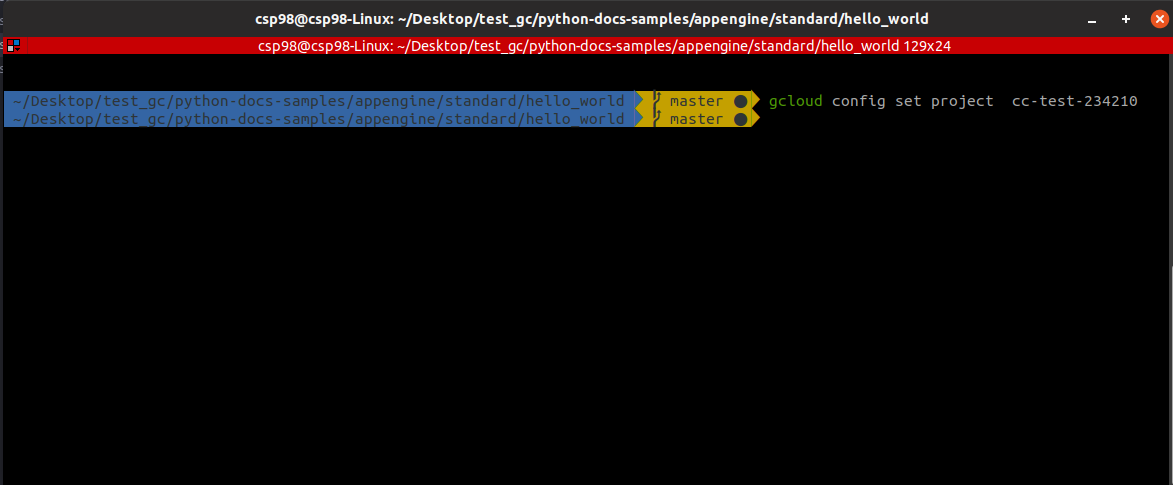
\includegraphics[scale=0.33]{img/tutorial/3setproject}
    \end{figure}
\end{frame}

\begin{frame}[fragile]{Step 3: testing the app in the local machine}
    \begin{figure}[H]
      \centering
      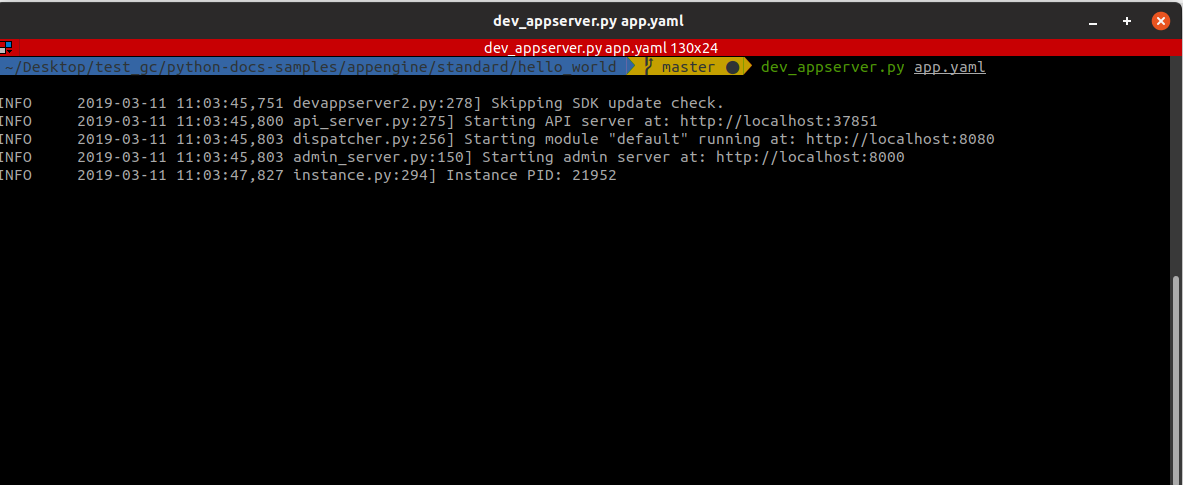
\includegraphics[scale=0.33]{img/tutorial/4localdeploy}
    \end{figure}
\end{frame}

\begin{frame}[fragile]{Step 3: testing the app in the local machine}
    \begin{figure}[H]
      \centering
      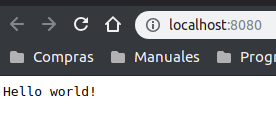
\includegraphics[scale=1]{img/tutorial/5localbrowse}
    \end{figure}
\end{frame}

\begin{frame}[fragile]{Step 4: modifying the app}
    \begin{figure}[H]
      \centering
      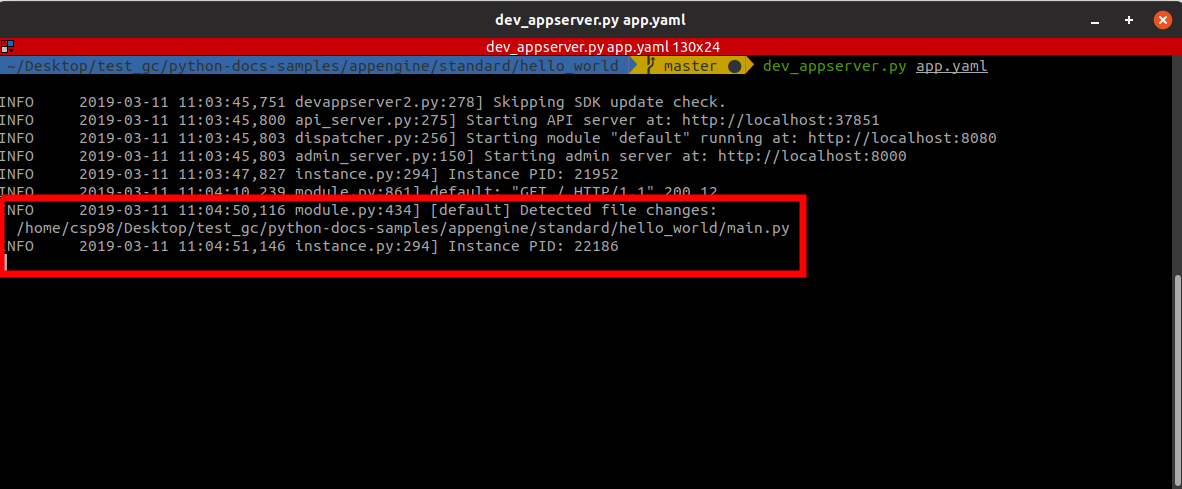
\includegraphics[scale=0.33]{img/tutorial/6modify}
    \end{figure}
\end{frame}

\begin{frame}[fragile]{Step 4: modifying the app}
    \begin{figure}[H]
      \centering
      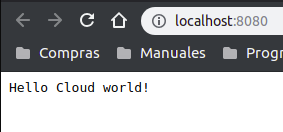
\includegraphics[scale=1]{img/tutorial/7browsemodify}
    \end{figure}
\end{frame}


\begin{frame}[fragile]{Step 5: deploying the app}
    \begin{figure}[H]
      \centering
      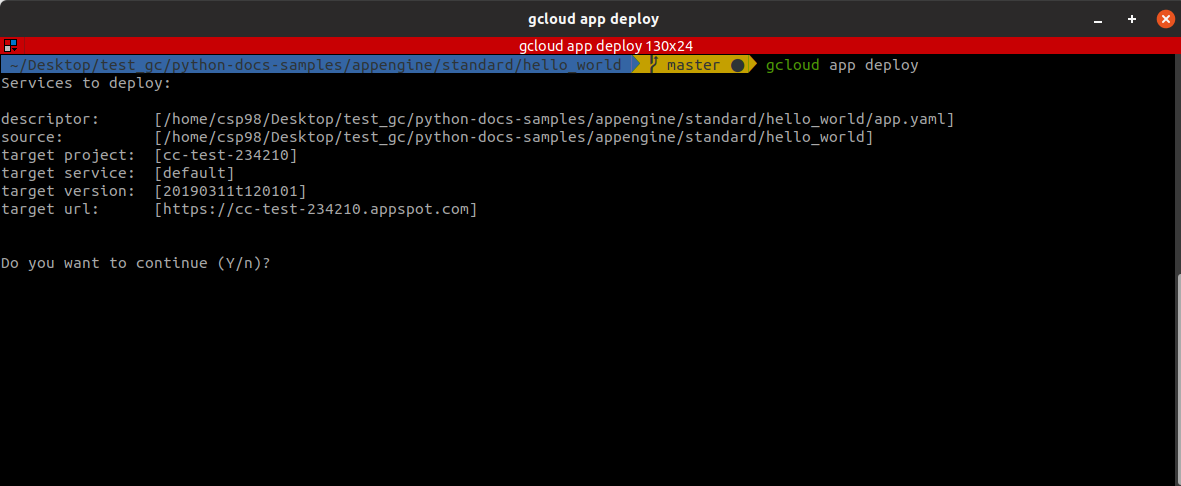
\includegraphics[scale=0.33]{img/tutorial/8deploy}
    \end{figure}
\end{frame}

\begin{frame}[fragile]{Step 5: deploying the app}
    \begin{figure}[H]
      \centering
      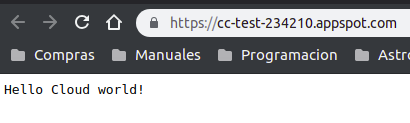
\includegraphics[scale=0.75]{img/tutorial/9browse}
    \end{figure}
\end{frame}

\begin{frame}[fragile]
 \begin{center}
  \Huge
  Thanks for your attention!
 \end{center}
\end{frame}

\end{document}
